\documentclass[graybox, envcountchap]{svmult}



\usepackage{mathptmx}        % selects Times Roman as basic font
\usepackage{amsmath}
\usepackage{amssymb}
\usepackage{color}
\usepackage{helvet}          % selects Helvetica as sans-serif font
\usepackage{courier}         % selects Courier as typewriter font
\usepackage{dirtree}
%\usepackage{type1cm}        % activate if the above 3 fonts are 
                             % not available on your system

\usepackage{makeidx}        % allows index generation
\usepackage{graphicx}        % standard LaTeX graphics tool
                                            % when including figure files
\usepackage{subfig}

\usepackage{multicol}        % used for the two-column index
\usepackage[bottom]{footmisc}% places footnotes at page bottom

\usepackage{hyperref}        %for hyperlinks
\hypersetup{colorlinks=true,urlcolor=blue}

\usepackage[misc]{ifsym}

\makeindex             % used for the subject index
                       % please use the style svind.ist with
                       % your makeindex program


\begin{document}


%%%%%%%%%%%%%%%%%%%%%%%%%%%%%%%%%%%%%%%%%%%%%%%%%%%%%%%%%%%%%%%%%



\title{Chapter Title}
% Use \titlerunning{Short Title} for an abbreviated version of
% your contribution title if the original one is too long
\author{First Author and Second Author}
% Use \authorrunning{Short Title} for an abbreviated version of
% your contribution title if the original one is too long
\institute{First Author (\Letter) \at Name, Address of Institute, \email{name@email.address}
\and Second Author \at Name, Address of Institute \email{name@email.address}}
%
% Use the package "url.sty" to avoid
% problems with special characters
% used in your e-mail or web address
%
\maketitle

\abstract{Each chapter should be preceded by an abstract (about 250 words) that summarizes the content. The abstract will not appear at the beginning of the chapter in the hard copy of the book. The abstract will appear only \textit{online} at \url{www.SpringerLink.com} and be available with unrestricted access. This allows unregistered users to read the abstract as a teaser for the complete chapter.}





%%%%%%%%%%%%%%%%%%%%%%%%%%%%%%%%%%%%%%%%%%%%%%%%%%%%%%%%%





\section{Section Heading}
\label{sec:1}

Use the template \emph{chapter.tex} together with the Springer document class svmult to style the various elements of your chapter content in the Springer layout. However, authors should not worry too much about the exact style, as this can be fixed by the Editorial Office in the preparation of the proof.



\subsection*{Key-points to have in mind}


\subsubsection*{Figures}

Colored figures are welcome in any standard format (jpg, tif, ppt, gif). If possible please provide the original figure in high resolution (300 dpi minimum). {\color{red}\bf Please do not forget to obtain permission in case the figure is from a published article}. For journals like ApJ, PRD, PRL, etc. you do not need the permission if you are an author of the article of the original figures, but for most journals you need the permission even if you are the author of those figures.



\subsubsection*{Submission}

Please submit source files, compiled pdf file of the chapter, and figure permissions to the editors of your book.

\vspace{0.3cm}

\textcolor{red}{\bf Author submission deadline: {\it [Submission Deadline]}}



\subsubsection*{arXiv Policy}

Authors can post their chapter on arXiv if they wish to do it. There is no embargo for the {\it submitted} version of the manuscript, while there is an embargo of 12~months from publication for the {\it accepted} version. In the case of a chapter of a book, authors can post on arXiv -- at any time -- the submitted version, which often corresponds to, or it is very close to, the accepted version because editors are supposed to invite experts on the topic of every chapter. In the comment field on arXiv, please write something like ``Invited chapter for the edited book {\it [Title of the book]} (Eds. {\it [Names of the Editors]}, Springer Singapore, expected in {\it [expected year of publication]})''. After the publication of the chapter, you may add the DOI on the arXiv page.





%%%%%%%%%%%%%%%%%%%%%%%%%%%%%%%%%%%%%%%%%%%%%%%%%%%%%%%%%





\section{Section Heading}
\label{sec:2}

We recommend to use the \verb|eqnarray| environment to typeset your equations, e.g.
\begin{eqnarray}
a \times b = c \nonumber\\
\vec{a} \cdot \vec{b}=\vec{c}
\label{eq:01}
\end{eqnarray}



\subsection{Subsection Heading}
\label{subsec:2}

This is a subsection.



\subsubsection{Subsubsection Heading}

This is a subsubsection.



% For figures use
%
\begin{figure}[b]
\sidecaption
% Use the relevant command for your figure-insertion program
% to insert the figure file.
% For example, with the graphicx style use
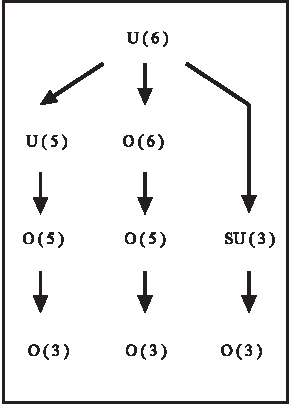
\includegraphics[scale=.95]{figure}
%
% If no graphics program available, insert a blank space i.e. use
%\picplace{5cm}{2cm} % Give the correct figure height and width in cm
%
\caption{If the width of the figure is less than 7.8 cm use the \texttt{sidecapion} command to flush the caption on the left side of the page. If the figure is positioned at the top of the page, align the sidecaption with the top of the figure -- to achieve this you simply need to use the optional argument \texttt{[t]} with the \texttt{sidecaption} command}
\label{fig:1}       % Give a unique label
\end{figure}



For typesetting numbered lists we recommend to use the \verb|enumerate| environment -- it will automatically render Springer's preferred layout.

\begin{enumerate}
\item{Livelihood and survival mobility are oftentimes coutcomes of uneven socioeconomic development.}
\begin{enumerate}
\item{Livelihood and survival mobility are oftentimes coutcomes of uneven socioeconomic development.}
\item{Livelihood and survival mobility are oftentimes coutcomes of uneven socioeconomic development.}
\end{enumerate}
\item{Livelihood and survival mobility are oftentimes coutcomes of uneven socioeconomic development.}
\end{enumerate}



For unnumbered list we recommend to use the \verb|itemize| environment -- it will automatically render Springer's preferred layout.

\begin{itemize}
\item{Livelihood and survival mobility are oftentimes coutcomes of uneven socioeconomic development, cf. Table~\ref{tab:1}.}
\begin{itemize}
\item{Livelihood and survival mobility are oftentimes coutcomes of uneven socioeconomic development.}
\item{Livelihood and survival mobility are oftentimes coutcomes of uneven socioeconomic development.}
\end{itemize}
\item{Livelihood and survival mobility are oftentimes coutcomes of uneven socioeconomic development.}
\end{itemize}



\begin{table}
\caption{Please write your table caption here}
\label{tab:1}       % Give a unique label
\begin{tabular}{p{2cm}p{2.4cm}p{2cm}p{4.9cm}}
\hline\noalign{\smallskip}
Classes & Subclass & Length & Action Mechanism  \\
\noalign{\smallskip}\svhline\noalign{\smallskip}
Translation & mRNA$^a$  & 22 (19--25) & Translation repression, mRNA cleavage\\
Translation & mRNA cleavage & 21 & mRNA cleavage\\
Translation & mRNA  & 21--22 & mRNA cleavage\\
Translation & mRNA  & 24--26 & Histone and DNA Modification\\
\noalign{\smallskip}\hline\noalign{\smallskip}
\end{tabular}
$^a$ Table foot note (with superscript)
\end{table}





%%%%%%%%%%%%%%%%%%%%%%%%%%%%%%%%%%%%%%%%%%%%%%%%%%%%%%%%%





\section{Section Heading}
\label{sec:3}

\begin{svgraybox}
If you want to emphasize complete paragraphs of texts we recommend to use the newly defined Springer class option \verb|graybox| and the newly defined environment \verb|svgraybox|. This will produce a 15 percent screened box 'behind' your text.

If you want to emphasize complete paragraphs of texts we recommend to use the newly defined Springer class option and environment \verb|svgraybox|. This will produce a 15 percent screened box 'behind' your text.
\end{svgraybox}



\begin{theorem}
Theorem text goes here.
\end{theorem}
%
% or
%
\begin{definition}
Definition text goes here.
\end{definition}



\begin{proof}
Proof text goes here.
\qed
\end{proof}





%%%%%%%%%%%%%%%%%%%%%%%%%%%%%%%%%%%%%%%%%%%%%%%%%%%%%%%%%





\begin{acknowledgement}
If you want to include acknowledgments of assistance and the like at the end of an individual chapter please use the \verb|acknowledgement| environment -- it will automatically render Springer's preferred layout.
\end{acknowledgement}





%%%%%%%%%%%%%%%%%%%%%%%%%%%%%%%%%%%%%%%%%%%%%%%%%%%%%%%%%





\section*{Appendix}
\addcontentsline{toc}{section}{Appendix}

When placed at the end of a chapter or contribution (as opposed to at the end of the book), the numbering of tables, figures, and equations in the appendix section continues on from that in the main text. Hence please \textit{do not} use the \verb|appendix| command when writing an appendix at the end of your chapter or contribution. If there is only one the appendix is designated ``Appendix'', or ``Appendix 1'', or ``Appendix 2'', etc. if there is more than one.





%%%%%%%%%%%%%%%%%%%%%%%%%%%%%%%%%%%%%%%%%%%%%%%%%%%%%%%%%





\biblstarthook{References should be \textit{cited} in the text by number.\footnote{Please make sure that all references from the list are cited in the text. Those not cited should be moved to a separate \textit{Further Reading} section.} The reference list should be \textit{sorted} in alphabetical order. If there are several works by the same author, the following order should be used: 
\begin{enumerate}
\item all works by the author alone, ordered chronologically by year of publication
\item all works by the author with a coauthor, ordered alphabetically by coauthor
\item all works by the author with several coauthors, ordered chronologically by year of publication.
\end{enumerate}
For the reference style, we suggest to use \textit{LaTeX (US)} from INSPIRE.}

\begin{thebibliography}{99}

%\cite{LIGOScientific:2016aoc}
\bibitem{LIGOScientific:2016aoc}
B.~P.~Abbott \textit{et al.} [LIGO Scientific and Virgo],
%``Observation of Gravitational Waves from a Binary Black Hole Merger,''
Phys. Rev. Lett. \textbf{116}, no.6, 061102 (2016)
doi:10.1103/PhysRevLett.116.061102
[arXiv:1602.03837 [gr-qc]].
%7349 citations counted in INSPIRE as of 06 Jan 2022

%\cite{Einstein:1916vd}
\bibitem{Einstein:1916vd}
A.~Einstein,
%``The Foundation of the General Theory of Relativity,''
Annalen Phys. \textbf{49}, no.7, 769-822 (1916)
doi:10.1002/andp.19163540702
%1236 citations counted in INSPIRE as of 06 Jan 2022

%\cite{Hawking:1975vcx}
\bibitem{Hawking:1975vcx}
S.~W.~Hawking,
%``Particle Creation by Black Holes,''
Commun. Math. Phys. \textbf{43}, 199-220 (1975)
[erratum: Commun. Math. Phys. \textbf{46}, 206 (1976)]
doi:10.1007/BF02345020
%9331 citations counted in INSPIRE as of 06 Jan 2022

%\cite{Penrose:1969pc}
\bibitem{Penrose:1969pc}
R.~Penrose,
%``Gravitational collapse: The role of general relativity,''
Riv. Nuovo Cim. \textbf{1}, 252-276 (1969)
doi:10.1023/A:1016578408204
%1319 citations counted in INSPIRE as of 06 Jan 2022

\end{thebibliography}





%%%%%%%%%%%%%%%%%%%%%%%%%%%%%%%%%%%%%%%%%%%%%%%%%%%%%%%%%

\end{document}

